% 图 6.9 棒状分子：(a) 低温晶态规则阵列 (b) 向列相取向有序位置无序 (c) 高温各向同性液体
\documentclass[tikz,border=5pt]{standalone}
\usetikzlibrary{arrows.meta}
\usepackage{amsmath}
\usepackage{bm}
\usepackage{fontspec}
\setmainfont{Times New Roman}
\begin{document}
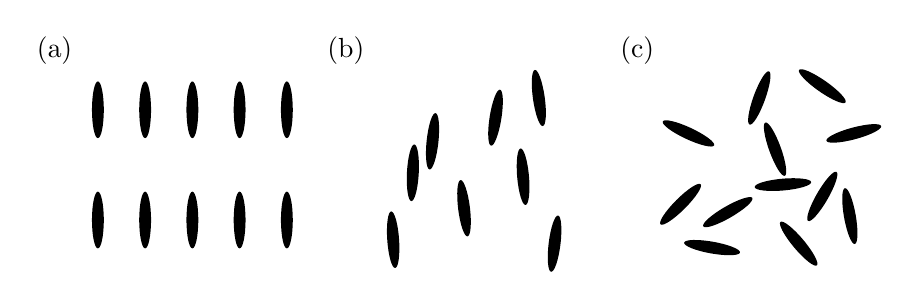
\begin{tikzpicture}[line width=0.8pt,>=Stealth]
\def\rod{\fill[black]}
% ---- (a) crystal: 5x2 regular array, all vertical ----
\begin{scope}[shift={(0,0)}]
\node at (-0.15,2.95) {(a)};
\foreach \i in {0,...,4}{\foreach \j in {0,1}{
  \fill ({0.4+\i*0.6},{0.8+\j*1.4}) ellipse (0.075 and 0.36);
}}
\end{scope}
% ---- (b) nematic: orientation ordered, positions disordered ----
\begin{scope}[shift={(3.7,0)}]
\node at (-0.15,2.95) {(b)};
\foreach \x/\y/\a in {0.45/0.55/4, 0.95/1.8/-6, 1.35/0.95/7, 1.75/2.1/-9,
                      2.1/1.35/5, 2.5/0.5/-7, 0.7/1.4/-3, 2.3/2.35/8}{
  \fill[rotate around={\a:(\x,\y)}] (\x,\y) ellipse (0.075 and 0.36);
}
\end{scope}
% ---- (c) isotropic liquid: random orientations, overlapping ----
\begin{scope}[shift={(7.4,0)}]
\node at (-0.15,2.95) {(c)};
\foreach \x/\y/\a in {0.5/1.9/65, 1.0/0.9/120, 1.6/1.7/20, 2.2/1.1/150,
                      0.8/0.45/80, 1.9/0.5/40, 2.6/1.9/105, 1.4/2.35/160,
                      2.55/0.85/10, 0.4/1.0/135, 1.7/1.25/95, 2.2/2.5/55}{
  \fill[rotate around={\a:(\x,\y)}] (\x,\y) ellipse (0.075 and 0.36);
}
\end{scope}
\end{tikzpicture}
\end{document}
